\section{Experiments}
\label{sec:exp}

\paragraph{Setup.}
We evaluate CLIP vision encoders fine-tuned on the task-arithmetic benchmark of
\citet{ilharco2023editing} as extended to twenty tasks by \citet{wang2024localizing}: all $190$
pairs over all $72$ linear modules for each ViT-B encoder, and $48$ \texttt{q}/\texttt{v} modules
for ViT-L/14.
$C_H$ comes from $1001$ images drawn round-robin across seven of the benchmark's own datasets on
the frozen base; a separate rebuilding record stores source counts, fold membership, and hashes.
All substantive overlap results use $k=8$. For whitening comparisons we truncate at the module's
participation ratio $m_{\rm white}$; the activation null retains $m_C=64$ eigendirections and
reads its rotation blocks from the eigenvalue standard errors as in \S\ref{sec:method}.
The calibration composition, not the calibration draw, is what moves the answer: a deliberately
different balanced MNIST/Cars/SVHN mixture gives $21.482\%$ ($-3.863$ points) while two
source-stratified refits at fixed source counts shift it by at most $0.243$ points
(Appendix~\ref{app:calibration}). The residual stays positive in both controls.
Brackets are finite-pool stability intervals, the $2.5$th and $97.5$th percentiles of $50{,}000$
crossed task--layer resampling replicates (seed $20260915$). They describe sensitivity to
reweighting the observed tasks and layers, not superpopulation coverage, and condition on one
checkpoint per task, fixed calibration and blocking, and the exact scalar null (or the pooled
$64$-draw Monte Carlo null for adapter arms). The external-reference \texttt{H0} is a separate
stress diagnostic and is never added to an estimate.

\begin{figure}[t]
\centering
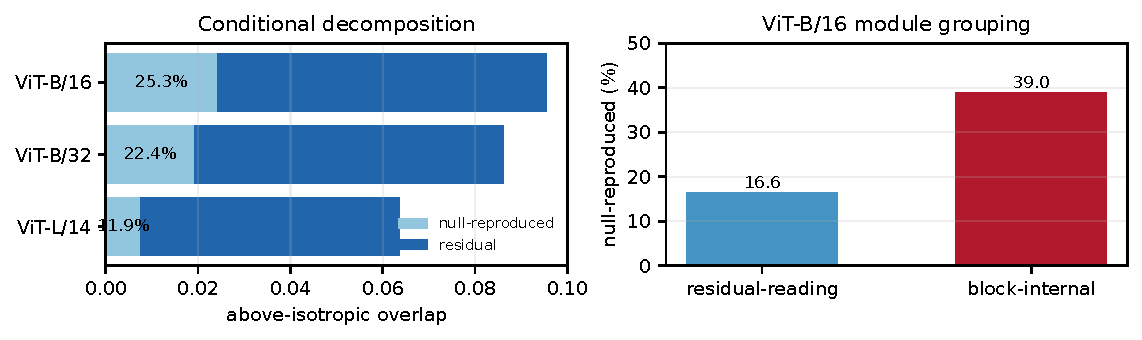
\includegraphics[width=\linewidth]{figures/fig_main.pdf}
\caption{Left: above-chance overlap split into the part the activation null reproduces and the
residual for each encoder. Right: an exploratory ViT-B/16 split by whether a module reads the
residual stream or a representation built within its block. All fractions use the null expectation
without adding the realised \texttt{H0} diagnostic.}
\label{fig:main}
\end{figure}

\subsection{Full fine-tuning: the conditional null reproduces about a quarter}
\label{sec:fullft}

In the two complete ViT-B measurements, the activation-conditioned null reproduces
$25.3451\%$ ($[19.3033,31.8010]$) and $22.3961\%$ ($[15.5516,29.8850]$) of above-isotropic
top-$8$ overlap. The partial ViT-L/14 \texttt{q}/\texttt{v} measurement gives $11.8961\%$
($[8.1064,16.4895]$).
Conditional on the fixed
null specification, the residual is positive under crossed task--layer resampling, but
should not automatically be identified with
task-derived sharing: it is directional agreement not accounted for by the conditioned
statistics. An earlier implementation put its headline reproduced fraction near $67\%$; the positive
control in \S\ref{sec:validate} shows why we reject it, with delivered-signal recovery of only
$45.6$--$51.7\%$ instead of the corrected null's $99.3$--$99.6\%$.

Module role, not architecture, is where the fraction actually moves, and the pooled headline hides
it. Figure~\ref{fig:main} shows the grouping: the exact null reproduces $16.6\%$ for ViT-B/16
modules reading the residual stream and $39.0\%$ for modules reading a representation built within
the block. Width carries part of that gap, since \texttt{fc2} has four times the input width and
supplies $81.9\%$ of the block-internal group's numerator. Holding width fixed leaves
\texttt{out\_proj} at $26.2\%$ against $16.1\%$ for attention \texttt{q}/\texttt{k}/\texttt{v}, so
roughly $10$ of the $22$ points survive as a role effect. One possible explanation is that
task-specific structure accumulates in the residual stream, whereas \texttt{out\_proj} and
\texttt{fc2} read representations more tightly constrained by the block.

The pooled ratio is a design-weighted blend, and its spread matters for how the headline is read.
Across the $72$ ViT-B/16 modules the reproduced fraction runs from $0.4\%$ to $65.1\%$ with median
$19.1\%$, and $394$ of $13{,}680$ cells have a negative residual. So $25.3\%$ is a property of this
module inventory, not of a typical module, and a different inventory would move it.

\begin{table}[h]
\centering
\caption{Cross-task read-subspace overlap and its scalar decomposition. Complete encoder pools use
all $190$ task pairs; the matched eight-task row uses all $28$. \texttt{raw} is
Eq.~\ref{eq:overlap}, \texttt{iso} is $k/d$, and \texttt{null} is the exact expectation in
Eq.~\ref{eq:null-expectation}. Terms are averaged before the ratio, and no Monte Carlo draw enters
these scalar results. The last column restricts every pool to \texttt{q} and \texttt{v}, the only
module set all three encoders share.}
\label{tab:main}
\small
\setlength{\tabcolsep}{4pt}
\begin{tabular}{@{}lrrrrrrr@{}}
\toprule
& modules & \texttt{raw} & \texttt{iso} & \texttt{null} & residual & reproduced & $q/v$ only \\
\midrule
ViT-B/16 & $72$ & $0.104574$ & $0.009115$ & $0.033309$ & $0.071265$ & $25.3\%$ & $14.7\%$ \\
ViT-B/32 & $72$ & $0.095313$ & $0.009115$ & $0.028420$ & $0.066893$ & $22.4\%$ & $13.5\%$ \\
ViT-L/14 $q/v$ & $48$ & $0.071402$ & $0.007813$ & $0.015377$ & $0.056024$ & $11.9\%$ & $11.9\%$ \\
matched FT8 $q/v$ & $24$ & $0.089930$ & $0.010417$ & $0.023333$ & $0.066597$ & $16.2\%$ & $16.2\%$ \\
\bottomrule
\end{tabular}
\end{table}

Table~\ref{tab:main} gives the terms behind these fractions, and its last column shows that most
of the apparent spread across encoders is module selection. ViT-L/14 is instrumented on \texttt{q}
and \texttt{v} only; restricting the two ViT-B pools to the same two module types moves them to
$14.7\%$ and $13.5\%$, so a $13.5$-point gradient becomes a $2.8$-point one. We therefore do not
read Table~\ref{tab:main} as an architecture trend. The fraction is also specification-dependent:
across $m_C\in\{16,32,64\}$ and $z\in\{1,2,3\}$ at $k=8$ it spans $20.22$--$25.61\%$ for ViT-B/16,
and $13.28$--$30.37\%$ once $k$ is swept as well, which changes the statistic rather than its
estimate (Appendix~\ref{app:calibration}).

The residual's sign is not in question and the resampling does not test it: every one of the $12$
layer margins ($\ge 0.0334$) and all $20$ task margins ($\ge 0.0282$) are strictly positive, so a
nonnegative reweighting cannot produce a negative replicate. What the intervals describe is width.
For ViT-B/16, ViT-B/32, and ViT-L/14 the crossed-resampling residual intervals are
$[+0.04540,+0.10568]$, $[+0.04224,+0.10085]$, and $[+0.03476,+0.08252]$. Within each replicate,
independent multinomial endpoint counts $C_t$ and layer counts $L_\ell$ give row weight
$C_aC_bL_\ell$; all module types in a layer stay together, weighted means precede the ratio, and
external \texttt{H0} diagnostics remain separate.

No single task or layer carries the result. Dropping one task at a time moves the reproduced
fraction within $24.685$--$25.896\%$, $21.856$--$22.939\%$, and $11.310$--$12.165\%$ for the three
encoders; dropping one layer at a time gives $24.359$--$28.411\%$, $21.272$--$26.392\%$, and
$10.955$--$13.587\%$. Every residual stays positive in every leave-one-out cell. The layer ranges
are the wider of the two, which is what the module-role split above predicts: layers differ in how
much of their width reads the residual stream.

\subsection{Low-rank adapters: a shared-start-compatible signature}
\label{sec:lora}

Low-rank adapters make the regime-specific conditioned object explicit. Since
$\mathrm{row}(BA)\subseteq\mathrm{row}(A)$, shared $A_0$ imposes a common admissible row space;
this remains exact when $A$ is frozen, while for trained $A$ we measure rather than assume it.
Across all $24$ targeted modules in the factor audit (Appendix~\ref{app:lora-factors}),
learned-from-zero $B$ overlaps at $0.0540$--$0.0570$, well below $A$'s
$0.8759$--$1.0000$ but still about five times chance. The
linearized pool, with bit-identical frozen $A$, has the highest $A$ and product overlap.
Almost all of that overlap is the rank constraint, and the null adds little to saying so. The
following pool-level estimates use all $24$ targeted modules and eight tasks. For LoRA-16 the
$A$-conditioned factor null reproduces $80.3\%$ ($[75.7,85.1]$) of above-isotropic overlap, and the
linearized pool $76.1\%$ ($[72.2,80.2]$). But a shared $A$ confines both updates to one
$r$-dimensional row space, where two independent top-$k$ subspaces already agree at $k/r$, and the
one-line comparator $(k/r-k/d)/(\overline{\texttt{raw}}-k/d)$ gives $82.0\%$ and $74.8\%$ on the same
pools. Conditioning on observed $A$ and on $B$'s spectrum therefore moves the answer by $1.7$ and
$1.3$ points. Under a shared start the admissible row space accounts for nearly all observed
product-subspace overlap, and the factor null confirms that rather than discovering it. Its
attainable plant delivers $37.4/49.8/57.0\%$ of the nominal increment with level-centred recovery
$101.1/101.1/100.7\%$ at $s=1/2/4$, so the construction is calibrated.

Full fine-tuning over the same $24$ modules gives $16.2\%$ ($[9.2,27.5]$). We do not read the gap
against $80.3\%$ as one contrast: they are ratios with different denominators, computed under nulls
that condition on different objects.

\paragraph{A regime-mismatched null changes the attribution.}
The activation null instead leaves $99.9\%$ of the same LoRA pool's above-chance overlap as
residual, versus $19.7\%$ under the observed-$A$-preserving factor null ($+0.5966$ versus
$+0.1176$). It answers a different question because it does not hold observed $A$ fixed;
transferring a null across regimes therefore changes the inferred effect size substantially.

\subsection{Consequences: attribution rather than a new merge}
\label{sec:projector}
\label{sec:merge}
\label{sec:ranking}
We rebuild the null-space projector of \citet{qiu2026nufilt} from real and independently
randomised task vectors (Appendix~\ref{app:projector}). Observed--null basis overlap is $0.8750$
versus $0.0208$ chance for LoRA and $0.2594$ versus $0.1667$ for full fine-tuning. The corresponding
basis mass in the top activation subspace is $0.1356$ and $0.2612$ (chance $0.0833$); none of
these projector statistics has a dedicated positive control. This does not test projector utility.
A separate cross-term-only compression heuristic does not beat the cumulative-update basis at any
rank budget, losing on $6$ to $8$ of the eight tasks from $r=32$ upward and tying within noise at
$r=8$ (Appendix~\ref{app:merge}). Calibration is also nearly rank-preserving over task pairs
(Spearman $0.994$--$0.995$); we do not test a retrained mergeability predictor. The contribution
is therefore inferential: a large effect or useful basis does not by itself establish the
mechanism invoked to explain it.
